\documentclass[a4paper, 11pt]{article} % Uses article class in A4 format

%----------------------------------------------------------------------------------------
%	FORMATTING
%----------------------------------------------------------------------------------------

\addtolength{\hoffset}{-2.25cm}
\addtolength{\textwidth}{4.5cm}
\addtolength{\voffset}{-3.25cm}
\addtolength{\textheight}{5cm}
\setlength{\parskip}{0pt}
\setlength{\parindent}{0in}

%----------------------------------------------------------------------------------------
%	PACKAGES AND OTHER DOCUMENT CONFIGURATIONS
%----------------------------------------------------------------------------------------

\usepackage{charter} % Use the Charter font
\usepackage[utf8]{inputenc} % Use UTF-8 encoding
\usepackage{microtype} % Slightly tweak font spacing for aesthetics

\usepackage[english]{babel} % Language hyphenation and typographical rules

\usepackage{algorithm}
\usepackage[noend]{algpseudocode}
\usepackage{amsthm, amsmath, amssymb} % Mathematical typesetting
\usepackage{float} % Improved interface for floating objects
\usepackage[final, colorlinks = true, 
            linkcolor = black, 
            citecolor = black]{hyperref} % For hyperlinks in the PDF
\usepackage{graphicx, multicol} % Enhanced support for graphics
\usepackage{color}
\usepackage{xcolor} % Driver-independent color extensions
\usepackage{marvosym, wasysym} % More symbols
\usepackage{rotating} % Rotation tools
\usepackage{censor} % Facilities for controlling restricted text
\usepackage{listings} % Environment for non-formatted code
\usepackage{pseudocode} % Environment for specifying algorithms in a natural way
\usepackage{booktabs} % Enhances quality of tables

\usepackage{cases}
\usepackage{bookmark}

\usepackage{tikz-qtree} % Easy tree drawing tool
\tikzset{every tree node/.style={align=center,anchor=north},
         level distance=2cm} % Configuration for q-trees

\usepackage[backend=biber,style=numeric,
            sorting=nyt]{biblatex} % Complete reimplementation of bibliographic facilities

\usepackage{csquotes} % Context sensitive quotation facilities

\usepackage[yyyymmdd]{datetime} % Uses YEAR-MONTH-DAY format for dates
\renewcommand{\dateseparator}{-} % Sets dateseparator to '-'

\usepackage{fancyhdr} % Headers and footers
\pagestyle{fancy} % All pages have headers and footers
\fancyhead{}\renewcommand{\headrulewidth}{0pt} % Blank out the default header
\fancyfoot[L]{} % Custom footer text
\fancyfoot[C]{} % Custom footer text
\fancyfoot[R]{\thepage} % Custom footer text

\newcommand{\note}[1]{\marginpar{\scriptsize \textcolor{red}{#1}}} % Enables comments in red on margin


\definecolor{codegreen}{rgb}{0,0.6,0}
\definecolor{codegray}{rgb}{0.5,0.5,0.5}
\definecolor{codemauve}{rgb}{0.58,0,0.82}

\lstset{ %
	language=python,                % choose the language of the code
	basicstyle=\footnotesize\ttfamily,       % the size of the fonts that are used for the code
	numbers=left,                   % where to put the line-numbers
	numberstyle=\tiny\color{codegray},      % the size of the fonts that are used for the line-numbers
	stepnumber=1,                   % the step between two line-numbers. If it is 1 each line will be numbered
	numbersep=5pt,                  % how far the line-numbers are from the code
	backgroundcolor=\color{white},  % choose the background color. You must add \usepackage{color}
	showspaces=false,               % show spaces adding particular underscores
	showstringspaces=false,         % underline spaces within strings
	showtabs=false,                 % show tabs within strings adding particular underscores
	frame=single,                   % adds a frame around the code
	tabsize=4,                      % sets default tabsize to 4 spaces  
	captionpos=b,                   % sets the caption-position to bottom
	breaklines=true,                % sets automatic line breaking
	breakatwhitespace=false,        % sets if automatic breaks should only happen at whitespace
	escapeinside={\%*}{*)},
	commentstyle=\color{codegreen},
	keywordstyle=\bfseries\color{magenta},
	stringstyle=\color{red},
	identifierstyle=\color{codemauve},
	keepspaces=true
}

%----------------------------------------------------------------------------------------

\begin{document}

%----------------------------------------------------------------------------------------
%	TITLE SECTION
%----------------------------------------------------------------------------------------

\fancyhead[C]{}
\hrule \medskip % Upper rule
\begin{minipage}{0.295\textwidth} % Left side of title section
    \raggedright
    DATA130008\\ % Your course code
    \footnotesize % Authors text size
    \hfill\\
    Introduction to Artificial Intelligence\\ % Your course name
\end{minipage}
\begin{minipage}{0.4\textwidth} % Center of title section
    \centering
    \Large % Title text size
    An $\alpha-\beta$ pruning approach to python-based Gomuku agent \\ % Assignment title and number
    \normalsize % Subtitle text size
\end{minipage}
\begin{minipage}{0.295\textwidth} % Right side of title section
    \raggedleft
    Shao Yanjun 19307110036\\
    Shao Yi 19307130113\\ % Your name
    \footnotesize % Email text size
    \hfill\\
    \today\\ % Date
\end{minipage}
\medskip\hrule % Lower rule
\bigskip

%----------------------------------------------------------------------------------------
%	ARTICLE CONTENTS
%----------------------------------------------------------------------------------------
\begin{multicols}{2}
    [
        \section{Introduction}
    ]

    \subsection{Gomoku}
    Gomoku, also called Five in a Row, is an abstract strategy board game. It is traditionally played with Go pieces (black and white stones) on a Go board. It is played using a 15×15 board while in the past a 19×19 board was standard. Within the Gomoku competition, however, we are assigned to develop some basic-level Gomoku agents on a 20×20 board for the sake of simplicity.
    
    Historically, researchers have been applying artificial intelligence techniques on playing gomoku for several decades. In 1994, L. Victor Allis raised the algorithm of proof-number search (pn-search) and dependency-based search (db-search), and proved that when starting from an empty 15×15 board, the first player has a winning strategy using these searching algorithms. This applies to both free-style gomoku and standard gomoku without any opening rules. It seems very likely that black wins on larger boards too.
    
    \begin{figure}[H]
    	\centering
    	\parbox{0.25\linewidth}{
    		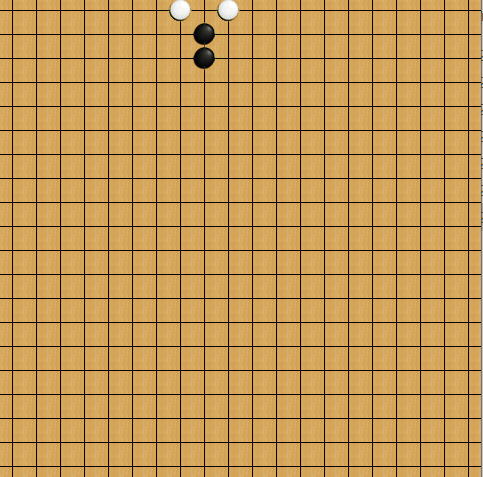
\includegraphics[width=\linewidth]{opening1.png}
    	}\quad
    	\parbox{0.25\linewidth}{
    		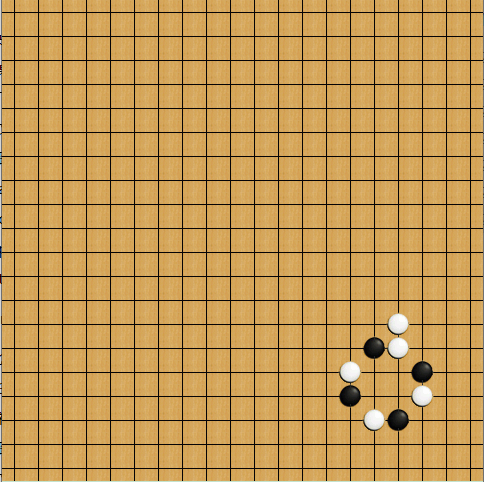
\includegraphics[width=\linewidth]{opening2.png}
    	}\quad
    	\parbox{0.25\linewidth}{
    		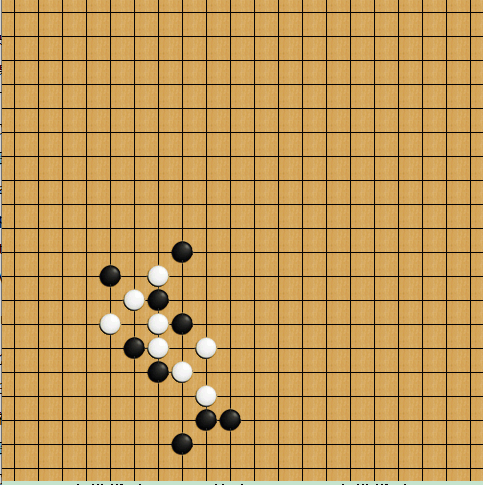
\includegraphics[width=\linewidth]{opening3.png}
    	}
    	\caption{Openings Overview}
    \end{figure}
    
    Therefore, hosts for contests came up with extra rules including Renju, Caro, Omok and Tournament Opening Rules. Renju, which is slightly different from traditional Freestyle Gomoku, bans the usage of three and three, four and four, and overlines applied to Black only. But our Gomoku contest provides 3 openings for each pair of AI under the rule of Freestyle Gomoku and generates a rating for every single participant. All ratings are calculated using Bayesian Elo with eloAdvantage =
    0, eloDraw = 0.01, and default prior.
    \subsection{$\alpha-\beta$ pruning}
    Alpha–beta pruning is a search algorithm that seeks to decrease the number of nodes that are evaluated by the minimax algorithm in its search tree.
    
	 \begin{figure}[H]
		\centering
		\parbox{0.25\linewidth}{
			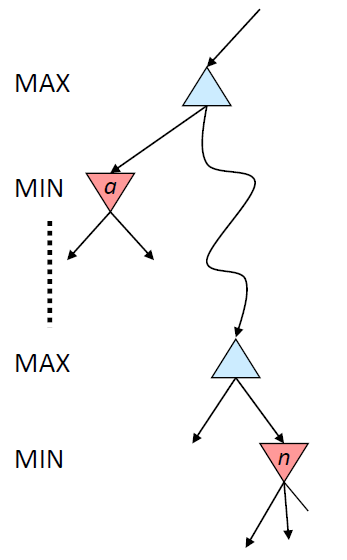
\includegraphics[width=\linewidth]{pruning.png}
		}
		\caption{$\alpha-\beta$ pruning}
	\end{figure}
	\begin{algorithm}[H]
		\caption{$\alpha-\beta$ Pruning Search}
		\small
		\begin{algorithmic}[1]
			\Function{\textsc{ALPHA-BETA-SEARCH}}{\textit{board}, \textit{color}} \textbf{returns} an action
			\State depth $\leftarrow$ 0
			\State v, action $\leftarrow$ \textsc{MAX-VALUE}(\textit{board}, \textit{color}, $-\infty$, $\infty$, \textit{depth})
			\State \textbf{return} action\\
			\EndFunction
		\end{algorithmic}
		\begin{algorithmic}[1]
			\Function{\textsc{MAX-VALUE}}{\textit{board}, \textit{color}, $\alpha$, $\beta$, \textit{depth}} \textbf{returns} v and action
			\If{TERMINAL-TEST(\textit{depth})} \textbf{return} UTILITY()
			\EndIf
			\State v $\leftarrow$ $-\infty$
			\For {\textbf{each} (x, y) in frontier}
			\State MOVE(\textit{board}, \textit{color}, \textit{(x, y)})
			\State move-v, move-action $\leftarrow$ MIN-VALUE(\textit{board}, \textit{opponent-color}, $\alpha$, $\beta$, \textit{depth+1})
			\If{move-v $>$ v} v $\leftarrow$ move-v, action $\leftarrow$ a
			\EndIf
			\If{v $\ge$ $\beta$} \textbf{return} v and action
			\EndIf
			\State $\alpha$ $\leftarrow$ MAX($\alpha$, \textit{v})
			\EndFor
	 
			\State \textbf{return} action\\
			\EndFunction
		\end{algorithmic}
		\begin{algorithmic}[1]
			\Function{\textsc{MIN-VALUE}}{\textit{board}, \textit{color}, $\alpha$, $\beta$, \textit{depth}} \textbf{returns} v and action
			\If{TERMINAL-TEST(\textit{depth})} \textbf{return} UTILITY()
			\EndIf
			\State v $\leftarrow$ $\infty$
			\For {\textbf{each} (x, y) in frontier}
			\State MOVE(\textit{board}, \textit{color}, \textit{(x, y)})
			\State move-v, move-action $\leftarrow$ MAX-VALUE(\textit{board}, \textit{opponent-color}, $\alpha$, $\beta$, \textit{depth+1})
			\If{move-v $<$ v} v $\leftarrow$ move-v, action $\leftarrow$ a
			\EndIf
			\If{v $\le$ $\alpha$} \textbf{return} v and action
			\EndIf
			\State $\beta$ $\leftarrow$ MIN($\beta$, \textit{v})
			\EndFor
			
			\State \textbf{return} action\\
			\EndFunction
		\end{algorithmic}
	\end{algorithm}
	
\end{multicols}

\bigskip

%------------------------------------------------

\begin{multicols}{2}
    [
        \section{Main}
        In this section, we will have to delve deeper into the implementation of $\alpha-\beta$ pruning techniques. Some details about how to evaluate the board through Utility() and how to define the frontier of a min-max search is literally what we are going to discuss about.
    ]

    \subsection{Utility}
    xxxxx

    \subsubsection{First Subsubtask}
    xxxxx

    \subsection{Frontier}
    The frontier in a min-max tree directly determines the validity of the searching algorithm and the size of the searching tree. A trade-off being compelling, a good agent is obliged to select a bounded number of possible actions for the sake of high performance, while it is not supposed to leave out any of the optimal solutions.
    
    Through careful spectating of several classical Gomoku games, we heuristically claim that majority of meaningful actions for a specific board state stays within 2 reaches.
        
    \begin{figure}[H]
    	\centering
    	\parbox{0.5\linewidth}{
    		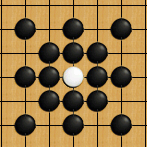
\includegraphics[width=\linewidth]{frontier.png}
    	}
    	\caption{2 reaches}
    \end{figure}
    
    However, if the agent is played on an aged CPU with unbearably high searching latency, we may make a small concession to half the frontier into 1 reach. 

\end{multicols}

\begin{multicols}{2}
	 [
		\section{Performance}
	]
	\subsection{Implementation}
	Unfortunately, our $\alpha-\beta$ pruning agent can only afford min-max search for $depth=1$. Two agents, \textit{pydan1-1} and \textit{pydan1-2}, namely depth-1 search with 1-reach frontier and 2-reach frontier, are implemented with the help of pyinstaller. 
	
	\subsection{Tournament}
	We conducted a tournament between \textit{pydan1-1}, \textit{pydan1-2} and the benchmark agent \textit{MUSHROOM}, and the results are as follows.
	\begin{figure}[H]
		\centering
		\parbox{1\linewidth}{
			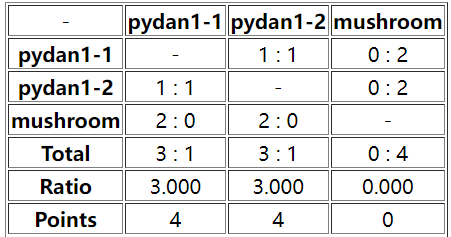
\includegraphics[width=\linewidth]{results.png}
		}

	\end{figure}
\end{multicols}

\begin{multicols}{2}
	[
	\section{Inspection of Future}
	]
	\subsection{AAA}
\end{multicols}



\bigskip

%----------------------------------------------------------------------------------------
%	REFERENCE LIST
%----------------------------------------------------------------------------------------

% \cite{Eureka}
% \printbibliography

%----------------------------------------------------------------------------------------

\end{document}